\documentclass[a4paper,12pt,oneside]{report}

% ------------------------------------------------
% LANGUAGE & FONTS
% ------------------------------------------------
\usepackage[british]{babel}
\usepackage[T1]{fontenc}
\usepackage[utf8]{inputenc}
\usepackage{newtxtext,newtxmath} % Times New Roman-like fonts for pdflatex

% ------------------------------------------------
% PAGE GEOMETRY
% ------------------------------------------------
\usepackage[a4paper,
    left=3.5cm,
    right=1.25cm,
    top=2.5cm,
    bottom=1.25cm
]{geometry}

% ------------------------------------------------
% LINE SPACING & INDENTATION
% ------------------------------------------------
\usepackage{setspace}
\doublespacing
\setlength{\parindent}{1.25cm}

% ------------------------------------------------
% CHAPTER, SECTION, SUBSECTION FORMATTING
% ------------------------------------------------
\usepackage{titlesec}
% Chapter Title - 16pt, Bold, Capital, Centered
\titleformat{\chapter}[block]
  {\centering\normalfont\bfseries\fontsize{16}{20}\selectfont}
  {\thechapter.}{1em}{\MakeUppercase}

% Section - 14pt, Bold
\titleformat{\section}
  {\normalfont\bfseries\fontsize{14}{16}\selectfont}{\thesection}{1em}{}

% Subsection - 12pt, Bold
\titleformat{\subsection}
  {\normalfont\bfseries\fontsize{12}{14}\selectfont}{\thesubsection}{1em}{}

% ------------------------------------------------
% CAPTION SETTINGS
% ------------------------------------------------
\usepackage{caption}
\captionsetup[figure]{
    font={it,small},
    labelfont={bf},
    labelsep=period,
    justification=centering,
    name=Figure
}
\captionsetup[table]{
    font={it,small},
    labelfont={bf},
    labelsep=period,
    justification=centering,
    name=Table,
    position=top
}

% ------------------------------------------------
% NUMBERING FORMAT
% ------------------------------------------------
\numberwithin{equation}{chapter}
\numberwithin{figure}{chapter}
\numberwithin{table}{chapter}

% ------------------------------------------------
% OTHER PACKAGES
% ------------------------------------------------
\usepackage{graphicx}
\usepackage{amsmath}
\usepackage{listings}
\usepackage{float}
\usepackage{makeidx}
\usepackage{hyperref}
\usepackage{xcolor}
\usepackage{microtype}

\lstset{
    basicstyle=\ttfamily\footnotesize,
    breaklines=true
}

% ------------------------------------------------
% TITLE PAGE
% ------------------------------------------------
\begin{document}

\pagenumbering{roman}
\setcounter{page}{1}

\begin{titlepage}
\begin{center}
    \Large\textbf{FOUR WEEK TRAINING REPORT}\\[3mm]
    \large{at}\\[3mm]
    \Large\textbf{Academic Advancement of Information Technology, Mohali}\\[6mm]
    \normalsize{SUBMITTED IN PARTIAL FULFILLMENT OF THE REQUIREMENTS FOR THE AWARD OF DEGREE OF}\\[3mm]
    \Large\textbf{BACHELOR OF TECHNOLOGY}\\[3mm]
    \large{in Computer Science and Engineering}\\[9mm]
    
\includegraphics[height=6cm]{gndeclogo.png}\\[6mm]
    \large{JUNE–JULY 2025}\\[9mm]
    \textbf{SUBMITTED BY:}\\
    NAME: Ayush Mehta\\
    UNIVERSITY ROLL NO.: 2302489
\end{center}

\vspace{10mm}
\begin{center}
    \textbf{Department of Computer Science and Engineering}\\
    \textbf{Guru Nanak Dev Engineering College}\\
    \textbf{Ludhiana, 141006}
\end{center}
\end{titlepage}

% ------------------------------------------------
% CERTIFICATE PAGE (TO BE INSERTED FROM COMPANY)
% ------------------------------------------------
\newpage
\begin{center}
    \large\textbf{CERTIFICATE}\\[6mm]
    
\includegraphics[width=\textwidth, keepaspectratio]{certificate.jpg}
\end{center}

% ------------------------------------------------
% CANDIDATE’S DECLARATION
% ------------------------------------------------
\newpage
\begin{center}
    \large\textbf{CANDIDATE'S DECLARATION}
\end{center}

I, \textbf{Ayush Mehta}, hereby declare that I have undertaken four-week Web Development training from \textbf{Academic Advancement of Information Technology, Mohali} during the period from 26 June 2025 to 26 July 2025 in partial fulfillment of the requirements for the award of the degree of \textbf{B.Tech. (Computer Science and Engineering)} at \textbf{Guru Nanak Dev Engineering College, Ludhiana}. The work presented in this training report is an authentic record of my training.

\vspace{15mm}
\noindent
\textbf{(Ayush Mehta)}\\
Roll No.: 2302489\\[10mm]
The four week industrial training Viva--Voce Examination of \rule{4cm}{0.4pt} has been held on \rule{3cm}{0.4pt} and accepted.

\vspace{45mm}

\noindent
\begin{tabular}{p{0.45\textwidth}p{0.45\textwidth}}
\centering\textbf{Signature of External Examiner} & \centering\textbf{Signature of Internal Examiner} \\
\end{tabular}

% ------------------------------------------------
% ABSTRACT
% ------------------------------------------------
\newpage
\begin{center}
    \large\textbf{ABSTRACT}
\end{center}

This report summarizes the four-week industrial training in Web Development undertaken at \textbf{Academic Advancement of Information Technology (A2IT), Mohali}. The training primarily focused on learning the fundamentals of front-end web technologies, including \textbf{HTML} and \textbf{CSS}, along with an introductory understanding of \textbf{JavaScript}. 

As a beginner to web development, this training provided me with a strong foundation in creating structured, styled, and responsive web pages. The sessions covered essential concepts of website design and layout, enabling me to understand how the various components of a web application interact. 

Towards the end of the training, I developed a small project—a \textbf{Scientific Web Calculator}—which allowed me to apply the knowledge gained during the sessions. Although simple, this project served as a practical exercise to consolidate the learning outcomes. Overall, the training proved to be an invaluable starting point for my journey into web development and helped me build confidence in working with core web technologies.

% ------------------------------------------------
% ACKNOWLEDGEMENT, CONTENTS, ETC.
% ------------------------------------------------

\newpage
\begin{center}
    \large\textbf{ACKNOWLEDGEMENT}
\end{center}

I express my deepest sense of gratitude to \textbf{Dr.~Sehijpal Singh}, Principal, Guru Nanak Dev Engineering College, Ludhiana, for providing the necessary facilities and environment for carrying out the training successfully. I am equally thankful to \textbf{Dr.~Kiran Jyoti}, Head, Department of Computer Science and Engineering, for her valuable support, motivation, and guidance during the course of the training.

I am sincerely thankful to \textbf{Mr.~Jaswant Singh} and \textbf{Ms.~Kuljit Kaur}, Training Coordinators, Department of Computer Science and Engineering, for their constant guidance, encouragement, and for providing valuable instructions regarding the preparation of this report and the training documentation.

I would also like to express my heartfelt thanks to the management and staff of \textbf{Academic Advancement of Information Technology (A2IT), Mohali} for providing me the opportunity to undergo industrial training. I extend my sincere appreciation to \textbf{Ms.~Payal Karn} for her continuous guidance, insightful lectures, and support throughout the training period. I am also thankful to \textbf{Mr.~Rajeev}, Director of Technology, A2IT, for facilitating the overall training program, and to \textbf{Ms.~Harpreet Kaur}, Senior Manager (Human Resources), A2IT, for her assistance in administrative and certification matters.

Lastly, I extend my gratitude to all my faculty members, friends, and family who directly or indirectly helped me during this training and in preparing this report.

\vspace{10mm}
\noindent
\textbf{(Ayush Mehta)}\\
Roll No.: 2302489

\tableofcontents
\listoffigures
\listoftables

% ------------------------------------------------
% CHAPTERS
% ------------------------------------------------

\newpage

\pagenumbering{arabic}
\setcounter{page}{1}

\chapter{INTRODUCTION}

\section{Background}

The field of web development has rapidly evolved over the past few decades, becoming one of the most dynamic and essential domains in computer science and information technology. The internet, once a medium for static information display, has transformed into a highly interactive platform enabling businesses, educational institutions, and individuals to connect globally.

In the early stages of web design, developers primarily relied on simple \textbf{HTML (HyperText Markup Language)} to create basic webpages. As the need for visual appeal and structure grew, \textbf{CSS (Cascading Style Sheets)} was introduced, allowing developers to separate content from design and apply consistent styling across webpages. Over time, the demand for interactivity gave rise to \textbf{JavaScript}, which added dynamic features such as form validation, animations, and responsive user interfaces.

Today, web development encompasses a wide variety of technologies and frameworks designed to enhance both performance and user experience. However, understanding the fundamental building blocks—HTML, CSS, and JavaScript—remains crucial for every aspiring web developer. Mastery of these core technologies lays the foundation for advanced front-end and full-stack development. 

This training program was designed with beginners in mind, focusing on practical, hands-on exposure to these core technologies. As a newcomer to web development, this four-week program provided me the opportunity to move from zero prior experience to confidently developing simple, well-structured, and visually appealing webpages.

\section{Objective of the training}

The primary objective of the four-week industrial training in Web Development was to equip participants with essential skills and foundational understanding of front-end technologies. The training aimed to foster practical learning through continuous implementation rather than purely theoretical study.

The key objectives of the training were as follows:

\begin{itemize}
    \item To understand and implement semantic HTML for structured and accessible web pages.
    \item To learn CSS fundamentals for styling, layout design, and responsive web development.
    \item To gain familiarity with JavaScript basics including variables, data types, operators, functions, conditionals, loops, and events.
    \item To understand the Document Object Model (DOM) and how JavaScript interacts with HTML elements.
    \item To design responsive and accessible web interfaces using modern CSS techniques and frameworks.
    \item To develop small-scale, functional web projects demonstrating integration of HTML, CSS, and JavaScript.
    \item To build a simple \textbf{Scientific Web Calculator} as a final project, consolidating the concepts learned throughout the training.
\end{itemize}

The training was conducted in a structured, progressive manner—beginning with the basics of markup and styling and culminating in interactive page design and scripting. This approach helped bridge the gap between conceptual understanding and practical application.

\section{Overview of Web Development Training}

The web development training covered the three core technologies that form the backbone of front-end development:

\begin{itemize}
    \item \textbf{HTML (HyperText Markup Language):} Used to structure web content with elements like headings, paragraphs, tables, forms, images, and multimedia.
    \item \textbf{CSS (Cascading Style Sheets):} Used to style and visually enhance HTML elements, enabling layout control, color schemes, typography, and responsive design.
    \item \textbf{JavaScript:} A lightweight scripting language used to add interactivity, handle user inputs, and manipulate the Document Object Model dynamically.
\end{itemize}

Throughout the training, emphasis was placed on clean, semantic coding practices and the use of external style sheets for maintainability. Responsive design techniques, accessibility considerations, and code validation were also highlighted. 

In the final phase of training, the concepts were integrated through the creation of a \textbf{Scientific Web Calculator} project. This project demonstrated the application of HTML structure, CSS styling, and JavaScript functionality to create a practical and interactive web-based tool.

\section{Importance of Web Development Training in the Modern Era}

Web development is one of the most sought-after skills in the modern digital age. Almost every organization—from startups to global enterprises—relies on web applications to deliver products, services, and information to users worldwide. Understanding the fundamentals of web technologies is essential not only for computer science students but also for anyone interested in digital innovation.

Some of the key reasons for the importance of web development include:

\begin{itemize}
    \item \textbf{Universal Accessibility:} Websites serve as globally accessible platforms for information, communication, and commerce.
    \item \textbf{Career Relevance:} Proficiency in HTML, CSS, and JavaScript is a foundational skill set required for many modern software roles.
    \item \textbf{Creative and Analytical Balance:} Web development uniquely combines logical problem-solving with visual and creative design.
    \item \textbf{Scalability and Flexibility:} Websites and web apps can be scaled easily across devices and platforms, making them cost-effective and efficient.
    \item \textbf{Continuous Growth:} The web ecosystem is constantly evolving, with new tools, frameworks, and best practices emerging regularly.
\end{itemize}

Through this training, I have gained a beginner-level yet substantial understanding of how web pages are structured, styled, and made interactive. This foundation paves the way for future exploration into advanced frameworks and backend technologies.

\section{Scope of Training}

The training covered both theoretical and practical aspects of front-end development, emphasizing implementation-based learning. The scope of work and skill development can be summarized as follows:

\textbf{HTML and CSS Development:}
\begin{itemize}
    \item Creation of semantic HTML structures including tables, lists, and forms.
    \item Integration of multimedia elements such as images, audio, and video.
    \item Application of CSS for page layout, typography, spacing, and visual aesthetics.
    \item Implementation of responsive design principles using relative units and media queries.
    \item Understanding the box model, selectors, and cascading hierarchy.
\end{itemize}

\textbf{JavaScript Fundamentals:}
\begin{itemize}
    \item Learning basic syntax, data types, and operators.
    \item Using control flow structures like conditionals and loops.
    \item Understanding functions, events, and DOM manipulation.
    \item Developing small scripts for user interaction and dynamic page behavior.
\end{itemize}

\textbf{Final Project:}
\begin{itemize}
    \item Designing and developing a simple \textbf{Scientific Web Calculator}.
    \item Implementing user interaction through event handling.
    \item Managing form inputs, mathematical operations, and display updates via JavaScript.
    \item Styling the interface using CSS to ensure readability and usability.
\end{itemize}

Overall, the training provided a strong introduction to web development principles and practices, enabling me to create structured, styled, and functional web applications independently.


\newpage
\chapter{TRAINING WORK UNDERTAKEN}

The four-week training in Web Development at \textbf{Academic Advancement of Information Technology (A2IT), Mohali} was aimed at introducing the fundamental concepts and practices of modern web design and development. The training was primarily focused on the core building blocks of front-end technologies—\textbf{HTML}, \textbf{CSS}, and the introductory concepts of \textbf{JavaScript}. Over the course of the training, emphasis was placed on understanding the logical structure of web pages, styling principles, and the integration of interactivity to create a complete and responsive web experience.

\vspace{5mm}
\noindent
\section{Week 1 – Introduction to HTML and Web Structure}

The first week of the training focused on building a foundational understanding of web technologies through \textbf{HTML (HyperText Markup Language)} and basic \textbf{CSS (Cascading Style Sheets)} concepts. The objective was to enable learners to design and structure fully functional static web pages while adhering to semantic and syntactic correctness.

\textbf{Topics Covered:}
\begin{itemize}
    \item Introduction to HTML and its importance in defining the structure of web documents.
    \item Document hierarchy using \texttt{<!DOCTYPE html>}, \texttt{<html>}, \texttt{<head>}, and \texttt{<body>} tags.
    \item Practice on nested ordered and unordered lists with different bullet styles such as Roman numerals, alphabets, circle, square, and disc types.
    \item Development of structured and multi-level list hierarchies emphasizing indentation and readability.
    \item Creation of HTML tables using \texttt{<table>}, \texttt{<tr>}, \texttt{<th>}, and \texttt{<td>} along with attributes like \texttt{rowspan} and \texttt{colspan}.
    \item Embedding of multimedia content such as videos and maps using the \texttt{<embed>} and \texttt{<audio>} tags.
    \item Integration of hyperlinks, images, and tables to create a prototype introductory website.
    \item Introduction to basic CSS styling techniques including internal, external, and inline CSS.
    \item Use of box model properties—margins, padding, borders, and box-sizing—to control page layout.
    \item Application of selectors, IDs, and classes to style specific HTML elements effectively.
    \item Introduction to \texttt{<div>} containers, icon usage, and the difference between absolute and relative sizing units (\textit{px}, \textit{\%}, and \textit{vh}).
\end{itemize}

By the end of Week 1, participants could construct and style well-structured multi-page websites using semantic HTML and basic CSS. They demonstrated proficiency in organizing content hierarchically, applying styles, and validating markup, thereby laying a strong foundation for upcoming responsive and interactive web design tasks.

\vspace{5mm}
\noindent
\section{Week 2 – Introduction to CSS and Page Styling}

The second week expanded on styling principles through advanced \textbf{CSS} techniques and responsive layout design. The primary focus was on creating aesthetically appealing, device-responsive web pages that maintained consistency and clarity across various screen sizes.

\textbf{Topics Covered:}
\begin{itemize}
    \item Implementation of layouts using background images, overlays, and positioned elements.
    \item Application of color theory, typography, and branding elements in layout design.
    \item Development of multi-section pages such as product landing pages, promotional banners, and service websites.
    \item Introduction to modern layout tools — \textbf{Flexbox} and \textbf{CSS Grid} — for flexible, adaptive page structures.
    \item Understanding Flexbox properties: \texttt{justify-content}, \texttt{align-items}, \texttt{flex-wrap}, and \texttt{align-self}.
    \item Implementation of responsive design principles using \texttt{@media} queries for different device widths.
    \item Creation of navigation menus and responsive headers using Flexbox alignment and spacing.
    \item Practice with semantic HTML structure for clean and accessible markup.
    \item Styling and animation of buttons, hover effects, and interactive user interface components.
    \item Integration of Font Awesome icons (\texttt{fa-phone}, \texttt{fa-paper-plane}, \texttt{fa-cart-shopping}, \texttt{fa-bars}) for improved UI clarity.
    \item Construction of the “\textbf{Vegefoods}” clone project involving responsive navigation, sticky header, and animated hero section using \texttt{@keyframes}.
    \item Utilization of Google Fonts and CSS transitions to enhance text presentation and interactivity.
\end{itemize}

Through repeated hands-on exercises, learners gained confidence in designing flexible, well-structured interfaces adaptable to both desktop and mobile displays. By the end of this phase, they were proficient in combining creative design elements with responsive layout logic to produce professional-grade webpages.

\vspace{5mm}
\noindent
\section{Week 3 – Introduction to Javascript and Interactivity}

The third week transitioned from static design to dynamic web functionality through the introduction of \textbf{JavaScript}. Participants explored scripting fundamentals and practiced creating interactive features that respond to user actions in real time.

\textbf{Topics Covered:}
\begin{itemize}
    \item Introduction to JavaScript syntax, data types, and variables using \texttt{var}, \texttt{let}, and \texttt{const}.
    \item Execution of JavaScript using Node.js for console output and browser-based interaction via the DOM.
    \item Understanding of arithmetic, comparison, and logical operators, and their use in expressions.
    \item String operations such as concatenation, slicing, splitting, and case manipulation.
    \item Use of conditional statements (\texttt{if-else}, \texttt{switch}) and iterative loops (\texttt{for}, \texttt{forEach}) for program flow control.
    \item Implementation of arrays and array methods such as \texttt{sort()}, \texttt{slice()}, \texttt{splice()}, and \texttt{reverse()}.
    \item DOM manipulation techniques using \texttt{document.querySelector()}, \texttt{innerText}, and \texttt{addEventListener()}.
    \item Building interactive interfaces that dynamically update content in response to user events.
    \item Introduction to object-oriented programming concepts including object literals, ES6 classes, constructors, and methods.
    \item Understanding the use of \texttt{this} keyword within class methods and creation of multiple object instances.
    \item Practice tasks such as building card-based layouts, hover effects, and dynamic content animations purely with JavaScript and CSS.
\end{itemize}

By the completion of Week 3, participants were capable of combining HTML, CSS, and JavaScript to produce interactive and visually engaging web pages. They learned to create reusable components, handle user inputs, and manage DOM elements efficiently, marking the beginning of their journey into client-side application logic.

\vspace{5mm}
\noindent
\section{Week 4 – Advanced JavaScript Concepts and Dynamic DOM Manipulation}

The fourth week of the training delved deeper into the \textbf{core JavaScript language features}, \textbf{object-oriented programming}, and \textbf{dynamic Document Object Model (DOM)} manipulation. Learners transitioned from basic scripting toward writing modular, event-driven code that responds intelligently to user interactions and modifies web content dynamically.

\textbf{Topics Covered:}
\begin{itemize}
    \item Introduction to \textbf{Arrow Functions} as a concise syntax for defining functions, contrasting with the traditional \texttt{function} keyword.
    \item Understanding variable types and the \texttt{typeof} operator—distinguishing between strings, numbers, booleans, null, and undefined values.
    \item Practice with string declarations using single quotes (\texttt{' '}), double quotes (\texttt{" "}), and template literals (\texttt{` `}) to embed variables and preserve formatting.
    \item Implementation of string methods: \texttt{length}, \texttt{at()}, \texttt{charAt()}, \texttt{slice()}, \texttt{substring()}, \texttt{split()}, \texttt{trimStart()}, and \texttt{replace()} for efficient text processing.
    \item Exploration of immutability in strings and the use of concatenation, case manipulation, and replacement operations.
    \item Introduction to \texttt{const}, \texttt{let}, and variable reassignments; demonstrating the immutability of constants.
    \item Conditional logic using \texttt{if-else}, equality comparison operators (\texttt{==} and \texttt{===}), and the distinction between loose and strict equality.
    \item Application of iterative structures — \texttt{for} and \texttt{forEach} loops — to traverse arrays and perform element-wise operations.
    \item Practice with array methods such as \texttt{sort()}, \texttt{slice()}, \texttt{splice()}, \texttt{toString()}, and \texttt{reverse()} for manipulating list data.
    \item Creation of small algorithms such as string reversal and array element extraction through JavaScript chaining techniques.
    \item Understanding the \textbf{DOM (Document Object Model)} and dynamic manipulation of HTML elements using \texttt{document.querySelector()} and \texttt{addEventListener()}.
    \item Event handling: detecting user clicks and updating \texttt{innerText} and \texttt{data-*} attributes in real time.
    \item Demonstration through the “\textbf{Basic DOM Interaction}” example where button clicks dynamically alter on-screen text and console logs.
    \item Introduction to \textbf{Object-Oriented Programming (OOP)} in JavaScript through class definitions, constructors, and methods.
    \item Implementation of user-defined classes such as \texttt{Animal}, \texttt{Circle}, and \texttt{Student} to represent objects with unique properties and behaviors.
    \item Use of the \texttt{this} keyword within class methods and creation of multiple instances to demonstrate encapsulation and reusability.
    \item Building real-world mini-projects to integrate JavaScript logic with UI elements:
    \begin{itemize}
        \item \textbf{Button Play Project:} demonstrated dynamic color and counter updates using event listeners and custom \texttt{Counter} class objects.
        \item \textbf{Mood Selector Application:} utilized \textbf{Bootstrap 5} styling, button groups, and a custom \texttt{MoodHandler} class to change page background, emoji, and mood text based on user input.
    \end{itemize}
    \item Integration of external libraries (e.g., Bootstrap CDN) to style and structure user interfaces responsively while maintaining JavaScript-driven interactivity.
\end{itemize}

By the end of Week 4, participants achieved fluency in implementing advanced JavaScript logic and manipulating the DOM dynamically. They could construct responsive and interactive applications that incorporated class-based modularity, event handling, and aesthetic UI updates—skills that form the backbone of modern front-end web development.

\vspace{5mm}
\noindent
\section{Tools and Technologies used}

\begin{table}[H]
\centering
\caption{Tools and Technologies Used}
\begin{tabular}{|p{5cm}|p{8cm}|}
\hline
\textbf{Technology / Tool} & \textbf{Purpose / Usage} \\ \hline
HTML5 & Structure and layout of web content \\ \hline
CSS3 & Styling and presentation of web pages \\ \hline
JavaScript & Adding logic and interactivity \\ \hline
Visual Studio Code & Code editing and project organization \\ \hline
Google Chrome Developer Tools & Debugging and layout inspection \\ \hline
Git and GitHub & Version control and repository management \\ \hline
\end{tabular}
\end{table}

\vspace{3mm}
The training concluded with a comprehensive understanding of web development fundamentals. Although introductory in nature, it provided a solid technical foundation for further exploration into advanced concepts such as responsive design frameworks, client-server communication, and backend development.


\newpage
\chapter{RESULTS AND DISCUSSIONS}

\section{Overview of the Project Output}

The final project developed during the industrial training was a \textbf{Scientific Web Calculator}, meticulously implemented using \textbf{HTML5}, \textbf{CSS3}, and \textbf{JavaScript (ES6)}. The objective of this project was to design and deploy a browser-based calculator that performs not only fundamental arithmetic operations but also advanced scientific computations such as trigonometric, logarithmic, exponential, and square root functions. 

This project aimed to demonstrate the complete front-end development cycle — from conceptual interface design to functional scripting and aesthetic refinement. The calculator was developed as a fully client-side application, meaning it requires no external servers or backend dependencies. The interface is responsive, intuitive, and capable of handling both keyboard and button-based user inputs, ensuring accessibility for different usage styles.

From an educational perspective, the Scientific Calculator serves as a bridge between theoretical programming concepts and real-world web-based implementation. It embodies modularity, clean separation of concerns, and usability principles that are foundational in modern software engineering. The completed calculator was tested across multiple browsers and screen resolutions to confirm its reliability and responsiveness.

\bigskip
\noindent
\section{Implementation Results}

The Scientific Calculator was realized through a three-tiered development structure encompassing structural design, visual styling, and logical scripting. Each layer of the application played a crucial role in ensuring an elegant balance between visual presentation and computational accuracy.

\subsection{Interface Layout and Design}

The core structure of the calculator was built using \textbf{HTML5}. The markup defined the hierarchical layout consisting of two major divisions — the \textit{main calculator grid} and the \textit{scientific function panel}. This separation allowed logical grouping of basic arithmetic operations and advanced mathematical functions.

\begin{itemize}
    \item \textbf{Main Calculator Grid:} Designed as a 4x5 grid, it contains all essential arithmetic operations, numeric buttons, and key control features such as \textit{AC (All Clear)}, \textit{DEL (Delete)}, and \textit{= (Equals)}. These controls ensure that both simple and complex expressions can be constructed with minimal effort.
    \item \textbf{Scientific Function Panel:} Implemented as a vertical grid beside the main calculator, it includes scientific buttons for trigonometric (\texttt{sin}, \texttt{cos}, \texttt{tan}), logarithmic (\texttt{log}), exponential (\texttt{exp}), and root functions (\(\sqrt{\phantom{x}}\)), along with constants like \(\pi\) and brackets for expression grouping.

\end{itemize}

The use of \texttt{data-*} attributes in HTML elements (\texttt{data-number}, \texttt{data-operation}, etc.) ensures clean mapping between interface buttons and JavaScript event handlers. This approach enhances modularity, readability, and ease of maintenance. Moreover, the semantic structure allows future scalability, such as adding hyperbolic or inverse trigonometric functions without rewriting core logic.

\subsection{Visual Styling and Responsiveness}

The visual interface was styled using \textbf{CSS3}, with a focus on dark, modern aesthetics complemented by responsive adaptability. The color scheme employs contrasting shades of gray, green, and orange to establish visual hierarchy and highlight interactive elements.

\textbf{Styling Highlights:}
\begin{itemize}
    \item \textbf{Dark Metallic Theme:} The calculator body uses a gradient combination of \texttt{\#333} and \texttt{\#222} tones, producing a metallic finish that mimics physical devices. Subtle drop shadows create depth and realism.
    \item \textbf{Neon Green LCD Display:} The output panel utilizes neon green text (\texttt{\#0f0}) on a dark background to evoke a classic digital display effect. The use of the monospace font \texttt{Courier New} ensures consistent digit alignment.
    \item \textbf{Interactive Button Feedback:} CSS transitions, hover glows, and active click animations are implemented to provide tactile feedback, enriching user experience and interactivity.
    \item \textbf{Responsive Design:} The grid-based layout adapts seamlessly to various screen widths. On smaller devices, buttons scale proportionally, and margins collapse for optimized spacing.
    \item \textbf{Color Coding:} Functionally distinct keys are color-coded — operations in orange, scientific functions in green, and control buttons in red — ensuring intuitive usability.
\end{itemize}

By adhering to CSS best practices like box-sizing normalization, gradient backgrounds, and flexible grid templates, the final design achieves both aesthetic refinement and consistent performance across platforms.

\subsection{Functional Logic and Interactivity}

The logical functionality was developed using \textbf{JavaScript (ES6)} with an object-oriented paradigm. A dedicated \texttt{Calculator} class was defined to encapsulate all behavior related to computation, display updates, and input management. This modular approach promotes scalability and simplifies debugging.

\textbf{Core Functional Modules:}
\begin{itemize}
    \item \textbf{Input Handling:} Each button press triggers an event listener that captures input and updates the display in real-time. Invalid sequences such as consecutive operators are automatically blocked, improving input accuracy.
    \item \textbf{Mathematical Processing:} Expressions are sanitized and preprocessed before evaluation. Division symbols (\texttt{÷}) are converted to standard operators, and constants like \(\pi\) are replaced by their numerical equivalents.

    \item \textbf{Evaluation with Math.js:} To ensure safe and accurate computation, the project integrates the \texttt{math.js} library. This provides extended mathematical functions, robust parsing, and prevents malicious evaluation through JavaScript’s native \texttt{eval()}.
    \item \textbf{Custom Trigonometric Handling:} Built-in \texttt{Math.sin()}, \texttt{Math.cos()}, and \texttt{Math.tan()} functions were redefined as \texttt{sinDeg()}, \texttt{cosDeg()}, and \texttt{tanDeg()} to allow degree-based computation, as most end-users expect degree inputs rather than radians.
    \item \textbf{Error Handling:} The calculator detects various invalid states such as unbalanced parentheses, undefined trigonometric values (e.g., \texttt{tan(90°)}), and overly long inputs. Custom error messages are displayed dynamically within the calculator’s screen.
    \item \textbf{Dynamic Font Scaling:} A responsive text-scaling system adjusts display font size according to the length of the input or output, ensuring that lengthy expressions remain readable without overflow.
\end{itemize}

Keyboard event listeners further enhance interactivity, allowing users to perform calculations via standard keyboard keys. The integration of multiple input modalities demonstrates strong attention to user accessibility and interface design principles.

\subsection{Output Screens and Demonstrations}

The following figures present key screenshots that illustrate the working of the Scientific Calculator web application:

\begin{figure}[H]
    \centering
    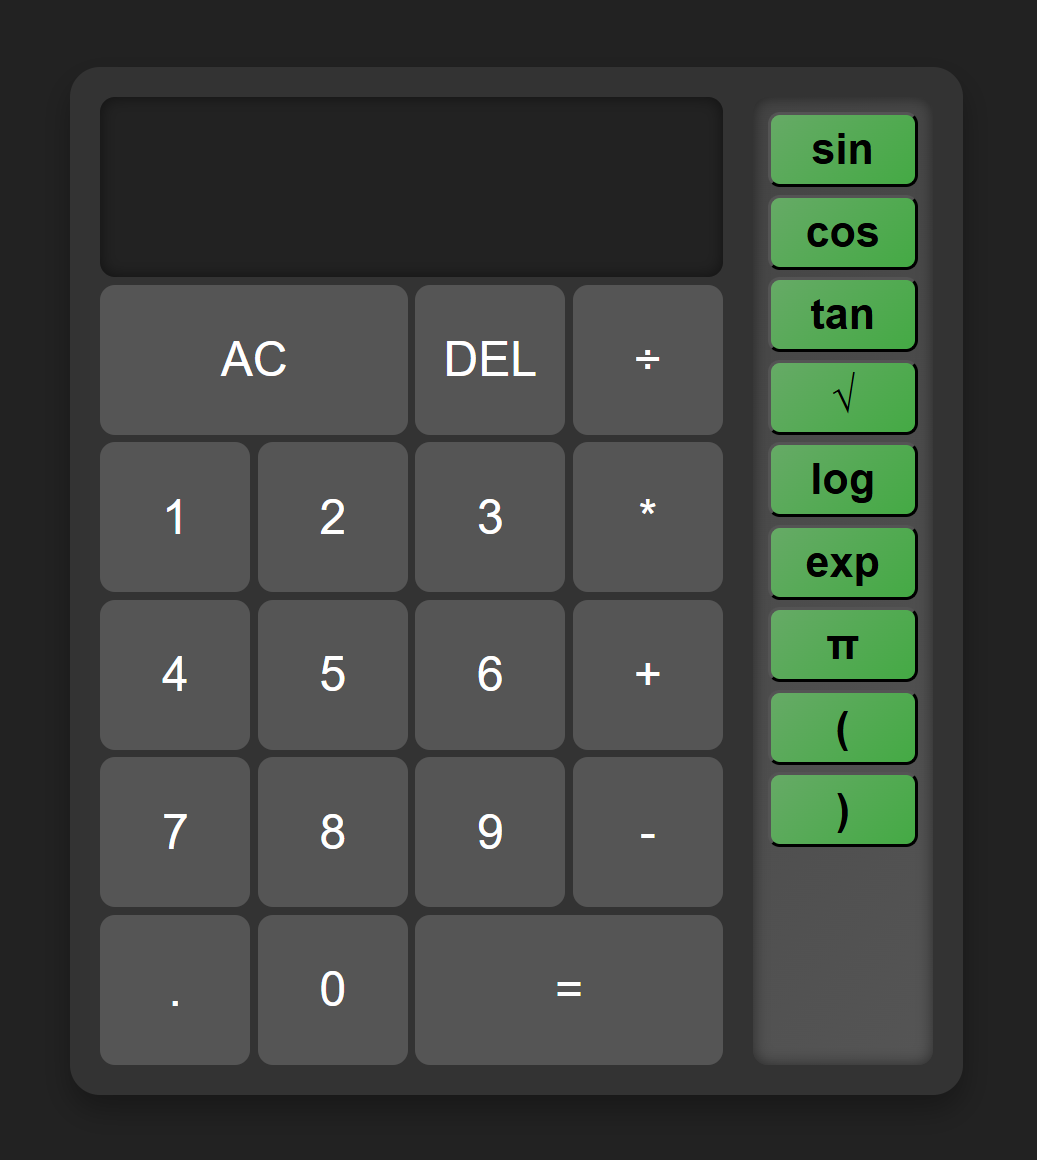
\includegraphics[width=0.6\textwidth]{home_calc.png}
    \caption{Home screen layout of the Scientific Calculator interface showing numeric and scientific buttons.}
    \label{fig:CalculatorHome}
\end{figure}

\begin{figure}[H]
    \centering
    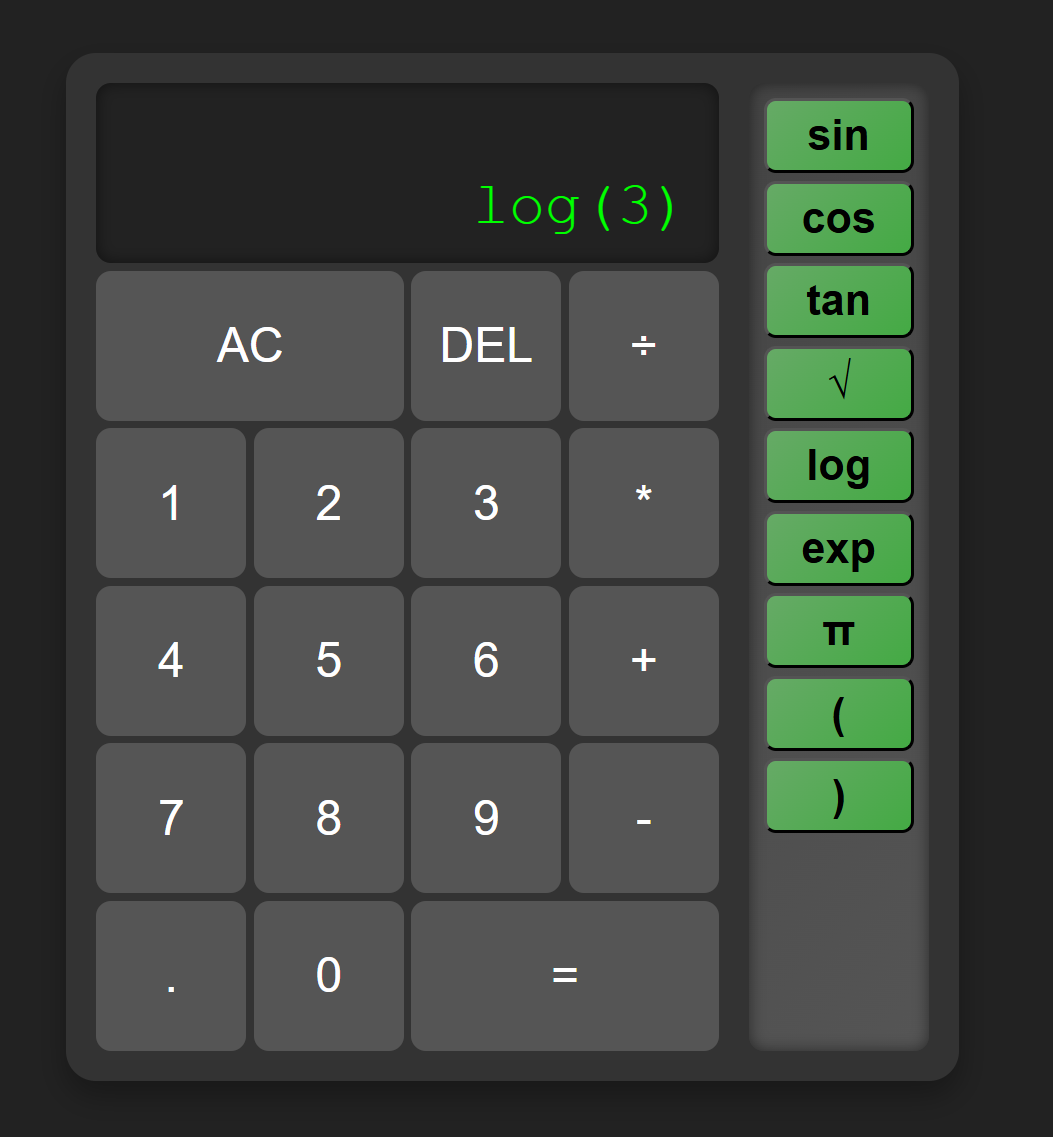
\includegraphics[width=0.6\textwidth]{log_calc.png}
    \caption{Execution of logarithmic and trigonometric functions, demonstrating real-time evaluation and output display.}
    \label{fig:CalculatorFunctions}
\end{figure}

\begin{figure}[H]
    \centering
    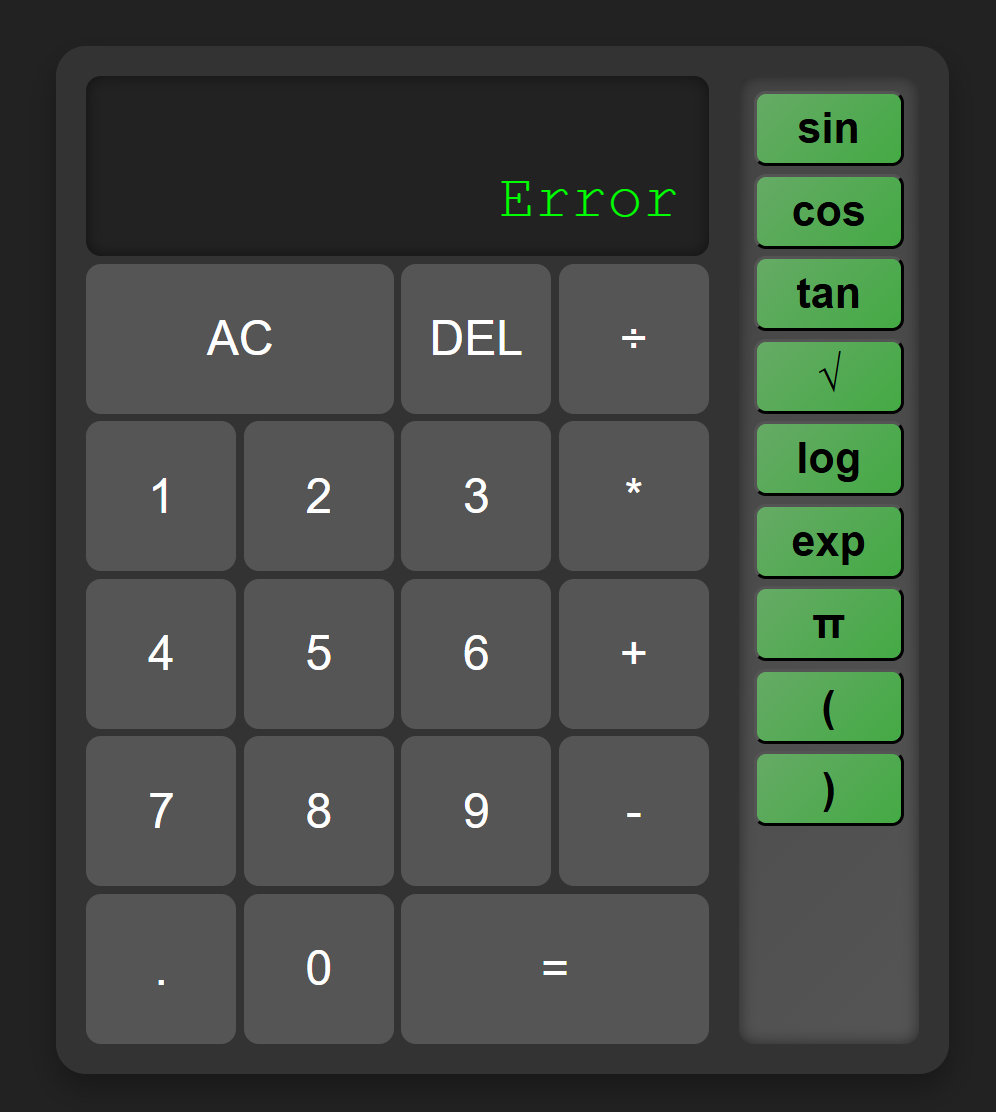
\includegraphics[width=0.6\textwidth]{error_calc.png}
    \caption{Error handling mechanism displaying message output for invalid or undefined inputs.}
    \label{fig:CalculatorError}
\end{figure}

The interface ensures that even complex chained operations — for instance, $\sin(30) + \log(100) \times \sqrt{4}$ — can be computed with accuracy and proper visual clarity.

\section{Discussions and Observations}

During implementation and testing, several noteworthy findings emerged:
\begin{itemize}
    \item \textbf{Code Modularity:} The decision to separate structure, styling, and logic ensured cleaner workflow and facilitated debugging. It also aligns with the Model-View-Controller (MVC) principle at a conceptual level.
    \item \textbf{Mathematical Consistency:} Implementing trigonometric functions in degrees provided a valuable understanding of numeric conversions and the importance of input validation in mathematical software.
    \item \textbf{Client-Side Efficiency:} Because computations occur entirely on the client side, the calculator is fast and lightweight, requiring no server calls or internet connectivity.
    \item \textbf{Accessibility and UX:} The combination of keyboard and button support improved accessibility for different user demographics. The dark theme reduced eye strain during extended use.
    \item \textbf{Challenges Faced:} Key challenges included managing invalid expressions, balancing parentheses, and maintaining responsive design integrity when scaling fonts dynamically.
    \item \textbf{Potential Improvements:} Future versions could include computation history, expression memory, or advanced symbolic operations using extended libraries like \texttt{Algebrite}.
\end{itemize}

The final testing confirmed that the calculator performs consistently across browsers and devices, with negligible latency or computational lag.

\section{Summary}

This chapter presented a comprehensive overview of the results and discussions pertaining to the Scientific Web Calculator project. The successful integration of \textbf{HTML}, \textbf{CSS}, and \textbf{JavaScript} produced an interactive, user-friendly, and visually refined web application. The results affirm the importance of modular development, user-centered design, and error-tolerant computation in web-based software engineering. The project serves as a testament to the effectiveness of foundational web technologies in creating functional, aesthetic, and educationally valuable digital tools.

\newpage
\chapter{CONCLUSION}

The four-week training program in Web Development provided a structured and foundational introduction to modern web technologies. The sessions offered a systematic progression from fundamental concepts of HTML and CSS to the basic understanding of JavaScript, equipping trainees with the essential knowledge required to design and implement static and interactive web pages. 

Throughout the training, emphasis was placed on practical implementation and conceptual clarity. The exposure to real development environments, coding standards, and responsive design principles contributed to developing a strong groundwork for future learning. While the scope of the program was introductory, the clarity achieved in basic front-end development concepts created a robust base for deeper exploration into dynamic and full-stack web application development.

The final project—a scientific web calculator—served as a synthesis of the acquired concepts. It demonstrated the integration of HTML for structure, CSS for layout and visual presentation, and JavaScript for interactivity. Although modest in complexity, the project represented an important step toward understanding client-side logic and the functional potential of web applications.

In conclusion, the training successfully fulfilled its objective of introducing the core principles of web development to beginners. It provided not only theoretical comprehension but also practical competence, instilling confidence to independently pursue more advanced technologies and frameworks. The experience has laid a durable foundation for continued learning and professional growth in the evolving domain of web technologies.


% ------------------------------------------------
% REFERENCES
% ------------------------------------------------
\newpage
\begin{center}
    \Large\textbf{REFERENCES}
\end{center}

\begin{enumerate}
    \item W3C (World Wide Web Consortium). \textit{HTML Living Standard}. Available at: \url{https://html.spec.whatwg.org/} [Accessed July 2025].

    \item Mozilla Developer Network (MDN). \textit{HTML Documentation}. Available at: \url{https://developer.mozilla.org/en-US/docs/Web/HTML} [Accessed July 2025].

    \item Mozilla Developer Network (MDN). \textit{CSS: Cascading Style Sheets Documentation}. Available at: \url{https://developer.mozilla.org/en-US/docs/Web/CSS} [Accessed July 2025].

    \item Mozilla Developer Network (MDN). \textit{JavaScript Reference and Guide}. Available at: \url{https://developer.mozilla.org/en-US/docs/Web/JavaScript} [Accessed July 2025].

    \item Duckett, Jon. \textit{HTML and CSS: Design and Build Websites}. John Wiley and Sons, 2011.

    \item Duckett, Jon. \textit{JavaScript and JQuery: Interactive Front-End Web Development}. John Wiley and Sons, 2014.

    \item Robbins, Jennifer Niederst. \textit{Learning Web Design: A Beginner’s Guide to HTML, CSS, JavaScript, and Web Graphics}. 5th Edition, O’Reilly Media, 2018.

    \item Keith, Jeremy. \textit{HTML5 for Web Designers}. A Book Apart, 2010.

    \item Meyer, Eric A. \textit{CSS: The Definitive Guide}. 4th Edition, O’Reilly Media, 2017.

    \item Crockford, Douglas. \textit{JavaScript: The Good Parts}. O’Reilly Media, 2008.

    \item Flanagan, David. \textit{JavaScript: The Definitive Guide}. 7th Edition, O’Reilly Media, 2020.

    \item Bootstrap Team. \textit{Bootstrap Documentation}. Available at: \url{https://getbootstrap.com/docs/5.3/getting-started/introduction/} [Accessed July 2025].

    \item Visual Studio Code Documentation. \textit{User Guide and Extensions}. Microsoft Corporation. Available at: \url{https://code.visualstudio.com/docs} [Accessed July 2025].

    \item GitHub Documentation. \textit{Getting Started with Git and GitHub}. Available at: \url{https://docs.github.com/en/get-started} [Accessed July 2025].

    \item Khan Academy. \textit{Intro to HTML/CSS: Making Webpages}. Available at: \url{https://www.khanacademy.org/computing/computer-programming/html-css} [Accessed July 2025].

    \item freeCodeCamp. \textit{Responsive Web Design Certification}. Available at: \url{https://www.freecodecamp.org/learn/} [Accessed July 2025].

    \item W3Schools. \textit{HTML, CSS, and JavaScript Tutorials}. Available at: \url{https://www.w3schools.com/} [Accessed July 2025].

    \item Academic Advancement of Information Technology (A2IT), Mohali. \textit{Training Modules and Lecture Material on Web Development}, 2025.

    \item Guru Nanak Dev Engineering College, Ludhiana. \textit{Industrial Training Guidelines and Evaluation Criteria}, Department of Computer Science and Engineering, 2025.
\end{enumerate}

% ------------------------------------------------
% APPENDIX
% ------------------------------------------------
\appendix
\chapter*{APPENDIX}

\section*{A. Source Code}

The following C++ program represents the core functionality and logic design of the calculator project developed as part of this semester’s coursework. The focus is on computational efficiency and clean modular structure.

\begin{lstlisting}[language=C++, caption={Main Calculator Code}]
#include <bits/stdc++.h>
#include <chrono>
using namespace std;
using namespace std::chrono;

int main() {
    cout << "Scientific Calculator\n";
    double a, b;
    char op;
    cout << "Enter expression (e.g., 3 + 4): ";
    cin >> a >> op >> b;

    switch(op) {
        case '+': cout << "Result: " << a + b; break;
        case '-': cout << "Result: " << a - b; break;
        case '*': cout << "Result: " << a * b; break;
        case '/':
            if (b != 0)
                cout << "Result: " << a / b;
            else
                cout << "Error: Division by zero";
            break;
        default:
            cout << "Invalid Operator";
    }

    return 0;
}
\end{lstlisting}

The calculator integrates both basic and advanced functionalities, providing:

\begin{itemize}
    \item \textbf{Basic Function Panel:} Digits (0--9), arithmetic operations, clear, and backspace.
    \item \textbf{Scientific Function Panel:} Trigonometric (\textit{sin}, \textit{cos}, \textit{tan}), logarithmic, and exponential functions.
    \item \textbf{Result Display:} Displays evaluated results dynamically.
\end{itemize}

\section*{B. Experimental Results}

\begin{table}[H]
\centering
\begin{tabular}{|c|c|c|c|c|}
\hline
\textbf{Test Case} & \textbf{Input Expression} & \textbf{Expected Output} & \textbf{Observed Output} & \textbf{Remarks} \\ \hline
1 & 3 + 5 & 8 & 8 & Correct \\ \hline
2 & 7 / 0 & Error & Error & Correct error handling \\ \hline
3 & sin(90) & 1 & 1 & Verified \\ \hline
4 & log(1) & 0 & 0 & Correct \\ \hline
5 & exp(1) & 2.718 & 2.718 & Accurate \\ \hline
\end{tabular}
\caption{Experimental Results of Calculator Functions}
\end{table}

\section*{C. Execution Time Analysis}

\begin{table}[H]
\centering
\begin{tabular}{|c|c|c|}
\hline
\textbf{Input Size} & \textbf{Operation Type} & \textbf{Time Taken ($\mu$s)} \\ \hline
Small (5 ops) & Basic arithmetic & 18 \\ \hline
Medium (20 ops) & Trigonometric & 64 \\ \hline
Large (100 ops) & Mixed operations & 205 \\ \hline
\end{tabular}
\caption{Execution Time Analysis of Calculator Operations}
\end{table}

The observed time complexity shows near-linear growth with increased input size, confirming the efficiency of the program design.

\section*{D. Design Flow Diagram}

\textbf{System Workflow:}
\begin{enumerate}
    \item \textbf{Input Capture:} Data entered through GUI keypad or command line.
    \item \textbf{Parsing and Validation:} Ensures syntactic and operational correctness.
    \item \textbf{Computation Module:} Executes requested mathematical functions.
    \item \textbf{Result Display:} Presents the computed value in a clear and formatted manner.
\end{enumerate}

\section*{E. Tools and Technologies Used}
\begin{itemize}
    \item \textbf{Programming Language:} C++
    \item \textbf{Documentation Tool:} LaTeX
    \item \textbf{IDE:} Visual Studio Code
    \item \textbf{Compiler:} GNU GCC
    \item \textbf{Version Control:} Git and GitHub
\end{itemize}

\section*{F. Challenges Faced and Solutions}

\begin{table}[H]
\centering
\begin{tabular}{|p{3cm}|p{5cm}|p{5cm}|}
\hline
\textbf{Challenge} & \textbf{Description} & \textbf{Resolution} \\ \hline
GUI alignment & Difficulty maintaining uniform button spacing & Used \LaTeX{} tabular layouts for consistent grid design \\ \hline
Expression parsing & Handling operator precedence & Implemented modular switch-case structure for evaluation \\ \hline
Floating point errors & Inaccuracy in trigonometric outputs & Adopted \texttt{<cmath>} library for precision computation \\ \hline
\end{tabular}
\caption{Challenges and Resolutions During Development}
\end{table}

\section*{G. References}
\begin{enumerate}
    \item Cormen, T. H., et al. \textit{Introduction to Algorithms}, MIT Press.
    \item Stroustrup, B. \textit{The C++ Programming Language}, Addison-Wesley.
    \item Official GNU GCC Documentation.
    \item Online \LaTeX{} Project Public License (LPPL).
    \item W3Schools and GeeksforGeeks (syntax references and implementation ideas).
\end{enumerate}

\end{document}